\setchapterstyle{lines}
\labch{appendix}

\setchapterstyle{lines}
\chapter{Analysis Checks}
\labch{analysis_checks}

\subsection{Asimov Inject/Recover Tests} \labsec{asimov_inject_recover_appendix}

\reffig{asimov_inject_recover_appendix} shows additional Asimov inject/recover tests for the \SI{0.3}{\gev} and\SI{1.0}{\gev} mass sets. The tests were described in \refsec{asimov_inject_recover}.

\begin{figure*}[h]
    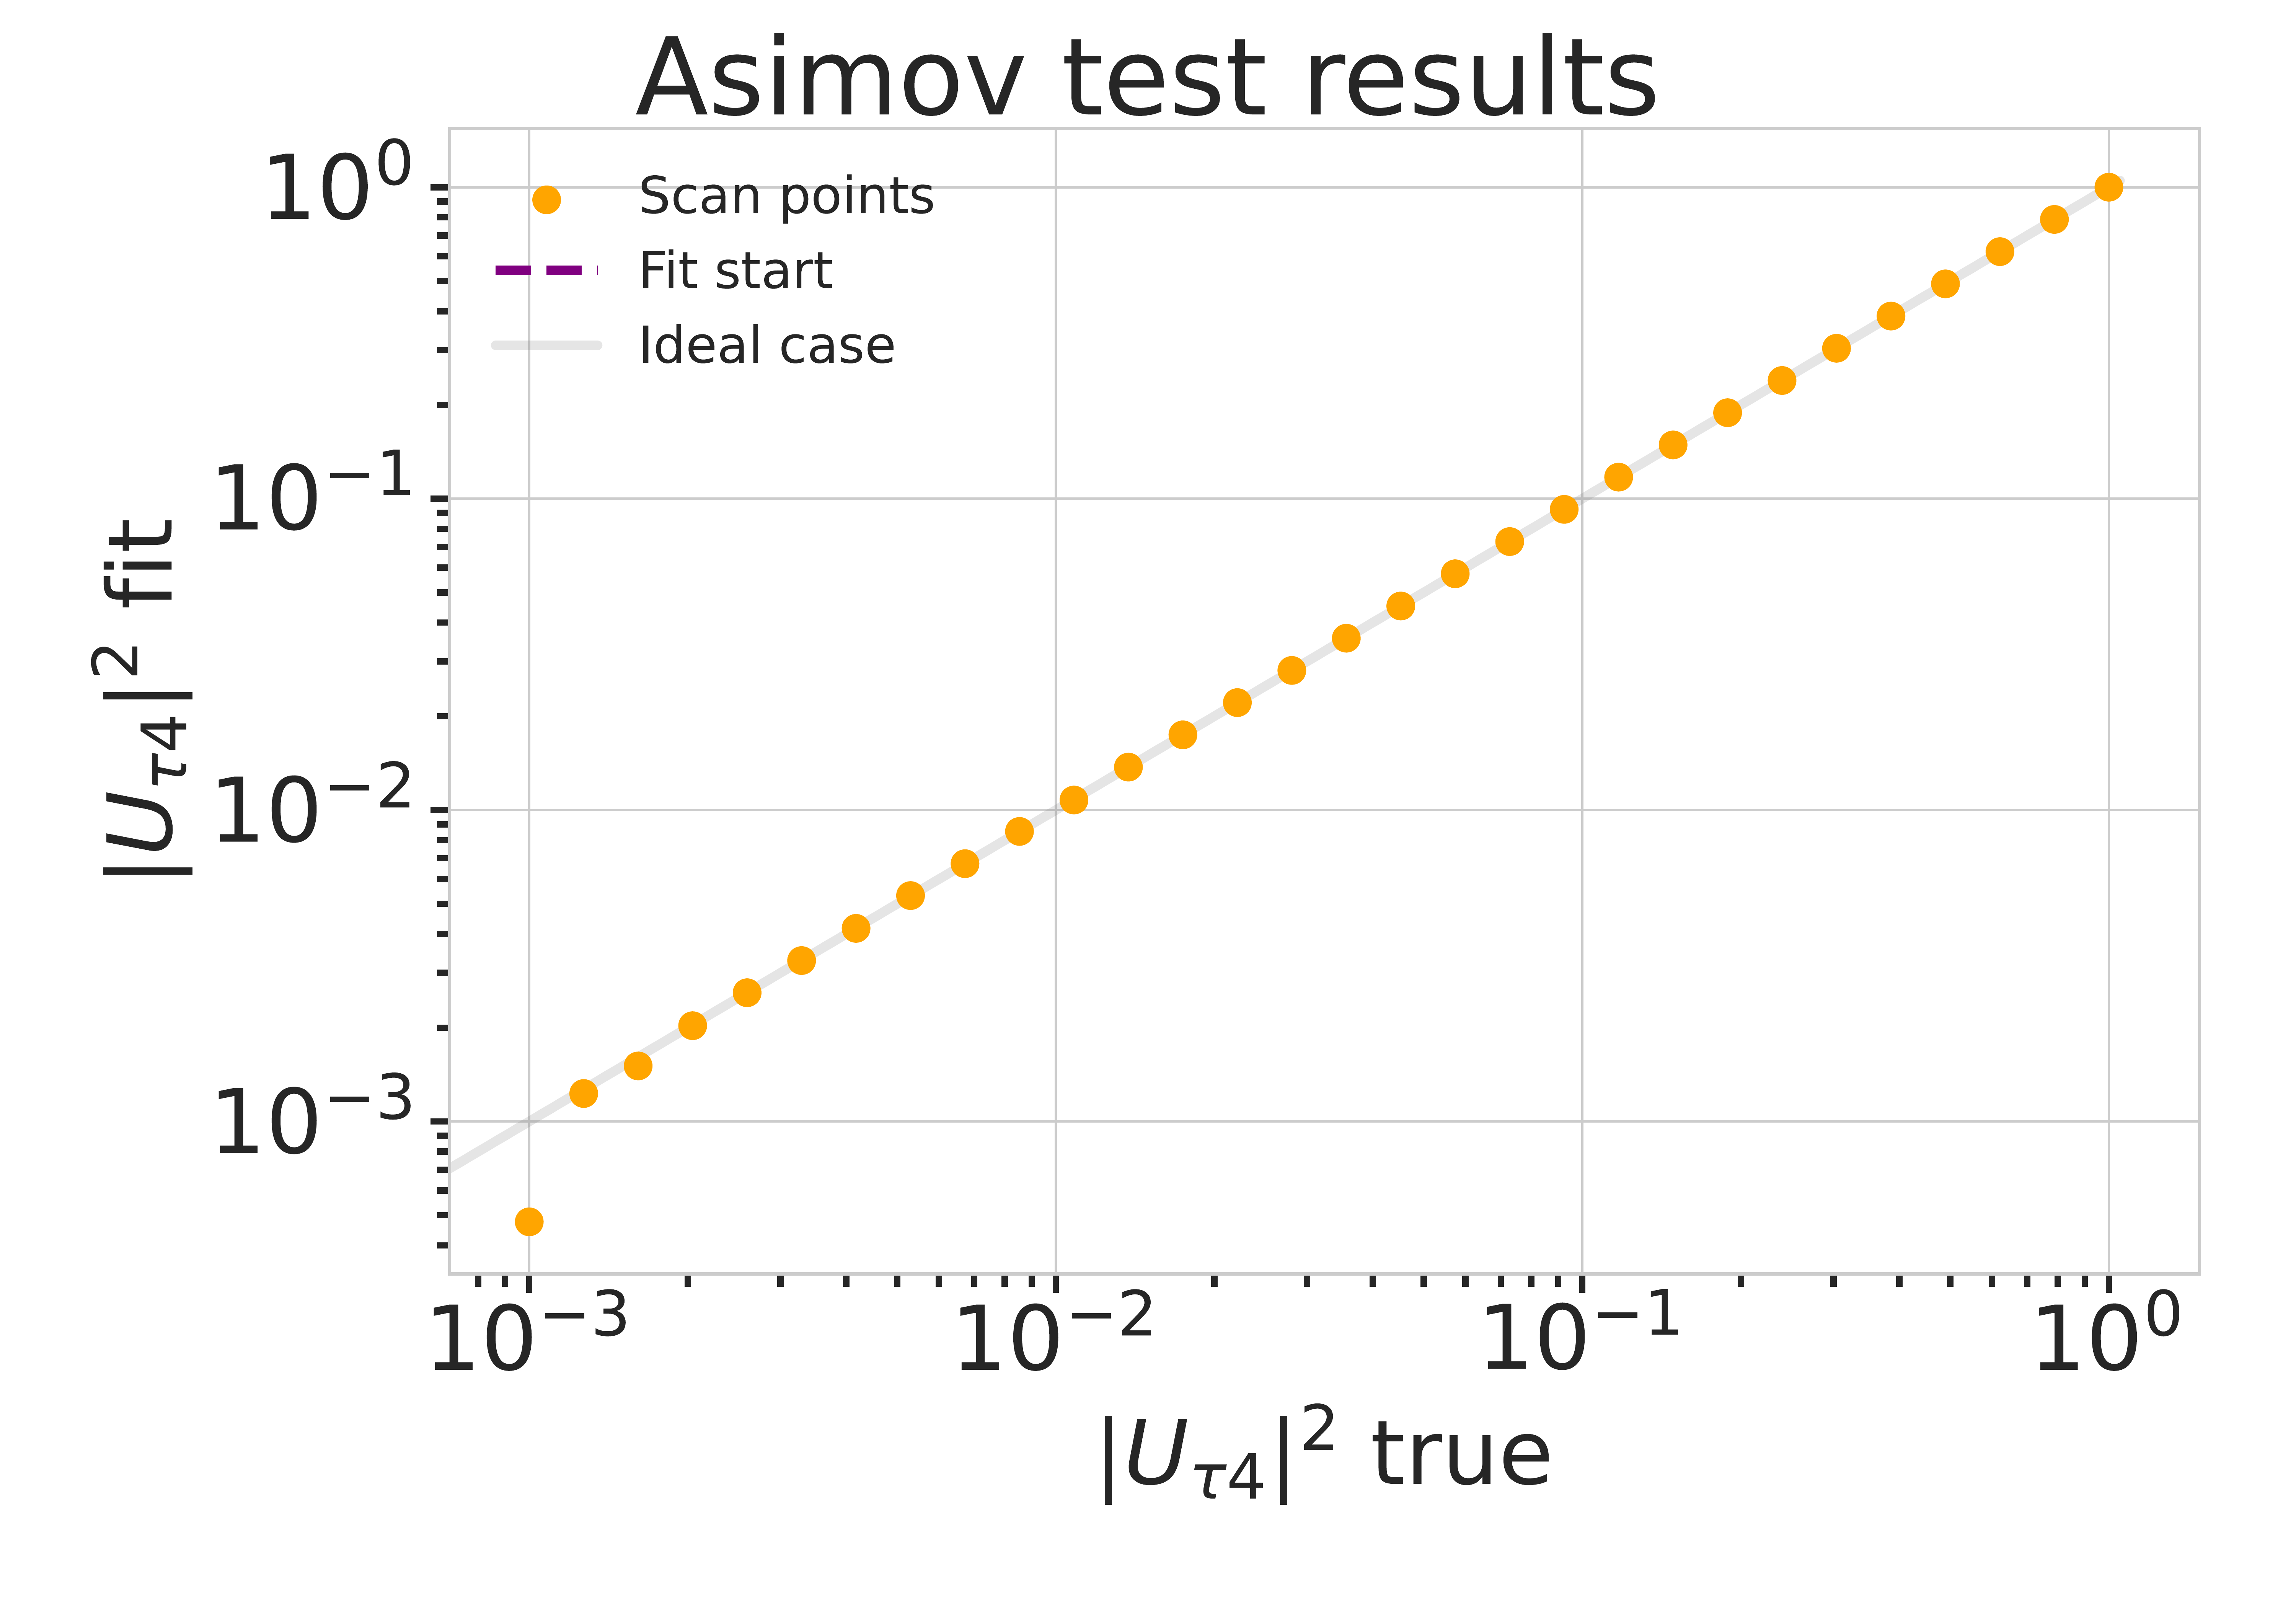
\includegraphics[width=0.49\linewidth]{figures/results/checks/asimov_scan_0.3_GeV-01.png}
    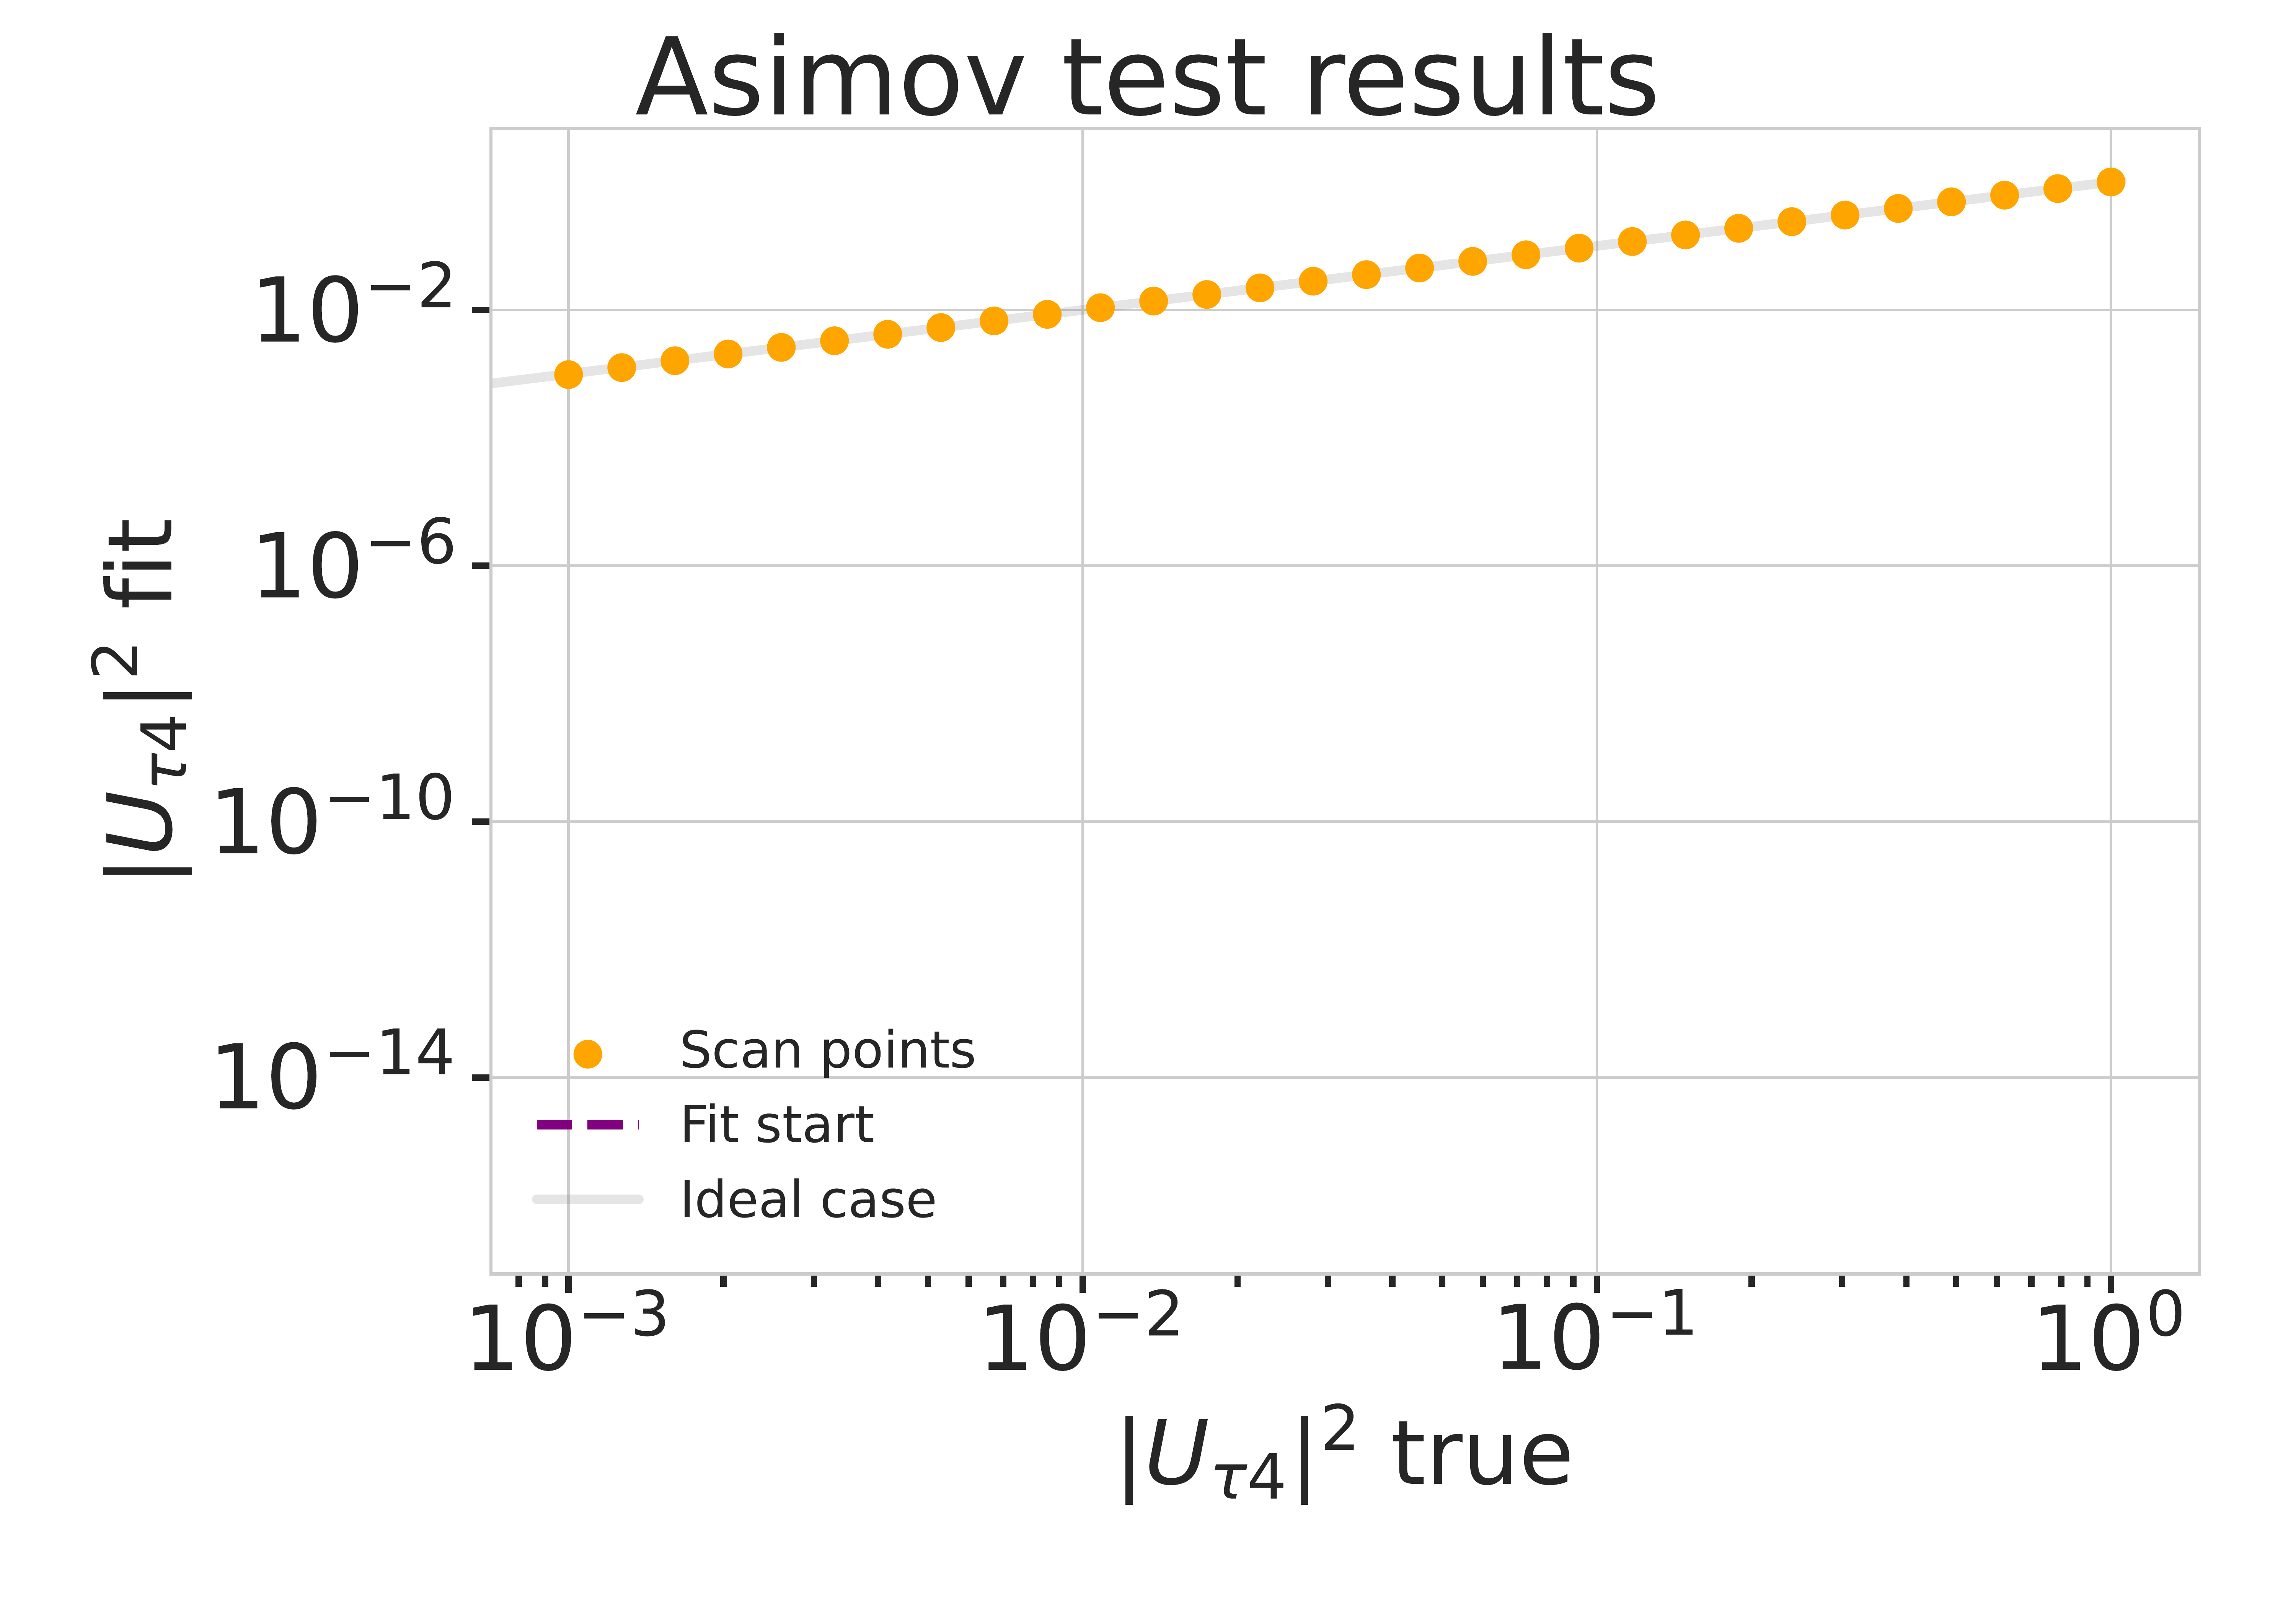
\includegraphics[width=0.49\linewidth]{figures/results/checks/asimov_scan_1.0_GeV-01.png}
	\caption[Asimov inject/recover test (\SI{0.3}{\gev}, \SI{1.0}{\gev})]{Asimov inject/recover test for the \SI{0.3}{\gev} (left) and \SI{1.0}{\gev} (right) mass sets. Mixing values between $10^{-3}$ and $10^{0}$ are injected and fit back with the full analysis chain. The injected parameter is always recovered within the statistical uncertainty.}
    \labfig{asimov_inject_recover_appendix}
\end{figure*}
